\section{Design}
The desing is the result of multiples discussions, were the goal was to provide a secure encrypted channel to transport the camera data from the top of the mountain to the enclave Embargo storage. Keep in mind that the data requires to flow from one site to another with a project time constrain of 7 seconds, making the task more interesting since now we need to encrypt the data before sending it to the other side of the tunnel, which takes a bit longer. 

In order to accomplish this challenge, and as mentioned before we choose the Arista DCS-7280CR3MK-32D4S with an encrypted module that could allow us to enable and setup IPSEC tunnels on top of the LHN. 
After Rubin purchased the equipment, two of them were sent to SLAC and the other two stayed at La Serena and then transported to the top of Cerro Pachón were the main telescope building and summit data center is located. These switches also work as our main TOR switches for the Rubin LFA cluster, same for SLAC and their Embargo storage cluster. This is made possible by using a mixture of MLAG + VVRP or VARP + OSPF.

\subsection{Hardware}
As was explained on \href{https://ittn-043.lsst.io/}{ittn-043}, the Rubin network is now using Arista Network as their core backbone equipment. As for the IPsec tunnels the hardware choosen was the Arista DCS-7280CR3MK-32D4S-R with an IPsec encryption module. 
To find the detailed datasheet please see the \href{https://www.arista.com/assets/data/pdf/Datasheets/7280R3-Data-Sheet.pdf}{Arista 7280R3 Data Sheet}.
The Arista 7280R3 Series with encryption delivers high performance, large packet buffers, high scale and availability with wire speed
AES-256-GCM encryption. 

\begin{itemize}
\item 32 x QSFP100, 4 x QSFP-DD
\item CPU Quad-Core x86
\item System Memory 64GB
\item Packet Buffer Memory 8GB
\item 1U
\item Wire speed L2 and L3 forwarding
\item Up to 4.8Tbps of wire speed performance with 8GB of buffer
\item Broad connectivity with 25G SFP, 100G QSFP and 400G OSFP / QSFP-DD
\item Encryption Support for TunnelSec (QSFP100 Ports)
\end{itemize}

\begin{figure}
    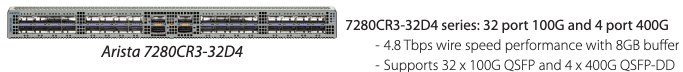
\includegraphics[width=16cm]{images/arista_datasheet01.png}
    \centering
    \caption{Arista DCS-7280CR3MK-32D4S}
  \end{figure}

There is a total of 4 Arista nodes, two of them are located in La Serena, Chile and the other two are at SLAC, US. 

\subsection{Licensing}

Arista has an easy way to manage their licenses and for the IPsec switches there are 3 main licenses that are running at this moment, been the IPsec license the most important one.

License feature: AHwSecSig
\begin{itemize}
\item License parameter:  *** info ommited *** 
\item Count: 1
\item Start: 2023-10-11 00:00:00
\item Expiration: 2123-09-17 00:00:00
\item Active: yes
\item License source: File
\end{itemize}

License feature: IPSec
\begin{itemize}
\item License parameter: None
\item Count: 4
\item Start: 2023-10-11 00:00:00
\item Expiration: 2123-09-17 00:00:00
\item Active: yes
\item License source: File
\end{itemize}

License feature: MACsec
\begin{itemize}
\item License parameter:  None
\item Count: 4
\item Start: 2023-10-11 00:00:00
\item Expiration: 2123-09-17 00:00:00
\item Active: yes
\item License source: File
\end{itemize}

The licenses were activated on all four switches, two of them in La Serena/Chile and the other two at SLAC/California and will not expire until 2123.

\subsection{Support}

Arista provides a TAC support team reachable via email, phone and online channels. We now have a good understanding on how to engage with them and scalate our issues. We have been working very closely to solve the many problems we encountered during the deployment of this project.
The Arista TAC team has proved to be an useful asset during the deployment of the IPsec tunnels environment.  

Note: The following definitions were extracted from the Arista official documentation from their latest release EOS64-4.32.1F that can be found \href{https://www.arista.com/en/um-eos/eos-data-plane-security#xx1009511}{here}

\newpage

\subsection{MLAG}
The Arista switches were configured in MLAG fashion to be used as TOR switches on both sites. Here a few benefits:

\begin{itemize}
    \item No wasted bandwidth with uplinks in Spanning Tree Blocking state
    \item Allows you to design non-blocking networks
    \item Maintains same level of resiliency with redundant paths available at all times
    \item No proprietary protocol used to connect an MLAG pair to servers or other switches. Interconnect to other switches or servers can use static LAG or IEEE 802.3ad LACP
    \item Spanning Tree Protocol can still be used in conjunction with MLAG to detect and handle any misconfigurations
\end{itemize}

\newpage

\subsubsection{Example of a MLAG configuration}
\begin{figure}
    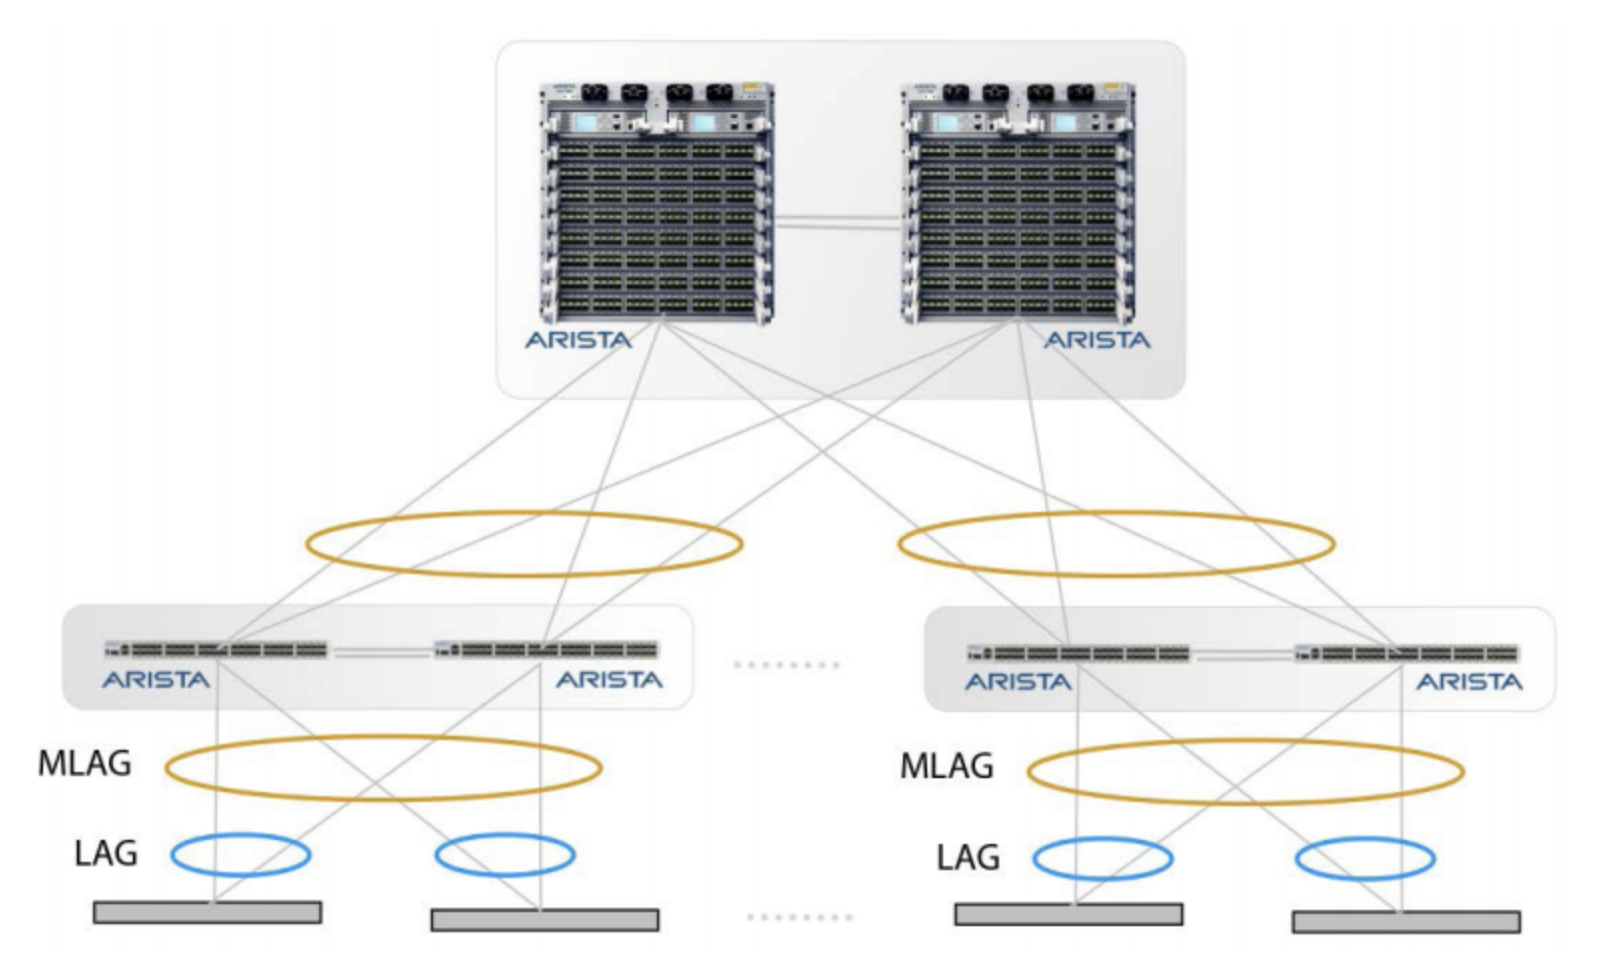
\includegraphics[width=16cm]{images/mlag.png}
    \centering
    \caption{Example of a MLAG configuration}
  \end{figure}

\subsection{IPSec}

The Arista DCS-7280CR3MK-32D4S provides IPSEC VTI mode which allows us to move the data using routing-based IPSEC, different from the conventional policy-based IPSEC.
The IPSec VTI tunnel mode support allows the customer to encrypt traffic transiting between two tunnel endpoints.

\begin{figure}
    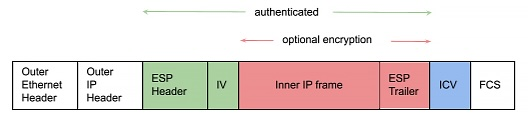
\includegraphics[width=16cm]{images/IPSEC_format.png}
    \centering
    \caption{IPSEC frame format}
  \end{figure}

\newpage

Internet Protocol Security (IPsec) is a protocol suite for securing Internet Protocol (IP) communications by authenticating and encrypting each IP packet of a communication session. IPsec includes protocols for establishing mutual authentication between agents periodically during the session and negotiation of cryptographic keys to be used during the session. IPsec supports network-level peer authentication, data origin authentication, data integrity, data confidentiality (encryption), and replay protection.
IPsec is used to protect data traffic between sites for example between Branch, HQ and Data center sites in an enterprise.
IPsec uses the following protocols to perform various functions:

\begin{itemize}
    \item Authentication Headers (AH): provides the connectionless integrity and data origin authentication for IP datagrams and provides protection against replay attacks.
    \item Encapsulating Security Payloads (ESP): provides the confidentiality, data-origin authentication, connectionless integrity and an anti-replay service (a form of partial sequence integrity).  
    Internet Key Exchange (IKE): is a key management protocol which provides security for virtual private networks' (VPNs) negotiations and network access to random hosts. It is also described as a method for exchanging keys for encryption and authentication over an unsecured medium, such as the Internet.
\end{itemize}
      
\subsection{Security Associations}
  
Security Associations (SA) provide the bundle of algorithms and data that provide the parameters necessary for AH and/or ESP operations. The Internet Security Association and Key Management Protocol (ISAKMP) provides a framework for authentication and key exchange, with actual authenticated keying material provided either by manual configuration with pre-shared keys, Internet Key Exchange (IKE and IKEv2) and other mechanisms. In order to decide what protection is to be provided for an outgoing packet, IPsec uses the Security Parameter Index (SPI), an index to the security association database (SADB), along with the destination address in a packet header, which together uniquely identify a security association for that packet. A similar procedure is performed for an incoming packet, where IPsec gathers decryption and verification keys from the security association database.
Full bidirectional communication requires at least two SAs, one for each direction. SA is defined by the following parameters:
  
\begin{itemize}
    \item Security Algorithms (AH) or Encapsulating Security Payloads (ESP) and keys.
    \item Mode: Tunnel or Transport.
    \item Key Management Method: Manual or IKE.
    \item Lifetime: Expressed in hours.
\end{itemize}
      
\subsection{Mode of Operation}
  
IPsec on Arista switches operates in tunnel mode. In tunnel mode, the entire IP packet is encrypted and/or authenticated. It is then encapsulated into a new IP packet with a new IP header.
  
Tunnel mode is used to create virtual private networks for network-to-network communications (for example, between routers to link sites). Tunnel mode is used for most network-to-network IPsec.

\subsection{Key Management}
  
Key management on Arista switches uses the Internet Key Exchange (IKE) method. Internet Key Exchange (IKE) supports automated generation and renegotiation of SAs (includes keys) between the devices at a configured interval so it is much more scalable and secure.  

IPsec needs SAs to define the algorithms and keys to use for protecting traffic. IKE establishes the SA so IPsec can protect traffic.
  
There are two IKE versions, IKEv1 and IKEv2. IKEv2 builds on IKEv1 but both are still widely used today.

\newpage

\subsubsection{IKEv1}
IKEv1 has two phases:
\begin{itemize}
    \item IKEv1 Phase 1
    \item IKEv1 Phase 2
\end{itemize}

\paragraph{IKEv1 Phase 1}
\begin{itemize}
    \item Uses main or aggressive mode exchange
    \item Negotiates IKE SA
    \item Used for control plane
    \item Peer authentication
\end{itemize}

\paragraph{IKEv1 Phase 2}
\begin{itemize}
    \item Uses quick mode exchange
    \item Negotiates IPsec SAs  
\end{itemize}
      
Note that there are two different SAs that are established. The IKE SA protects only the IKE key management session using the IKE policy defined. The policy should include the following parameters:
\begin{itemize}
    \item Encryption algorithm
    \item Hash MAC (HMAC) algorithm
    \item Peer authentication procedure
    \item Diffie-Hellman group for initial key exchange
    \item SA lifetime
\end{itemize}
          
IKE initially performs a Diffie-Hellman (DH) exchange at the start of the IKE session. A Diffie-Hellman (DH) exchange allows participants to produce a shared secret value. The strength of the technique is that it allows participants to create the secret value over an unsecured medium without passing the secret value through the wire. From that exchange, peers get shared keying material, which is then used for IKE encryption and integrity functions. The strength of that keying material can be used for faster performance, by choosing lower key sizes for Diffie-Hellman exchanges. The key length (strength) of Diffie-Hellman exchanges can be changed with the use of different DH groups.
  
When an IKE session's lifetime expires, a new Diffie-Hellman exchange is performed between peers and the IKE SA is re-established.
The IPsec protection policy resulting in IPsec SAs, defines the protection of network traffic. These IPsec SAs are usually negotiated over IKE sessions. The parameters that define the IPsec protection policy are:
\begin{itemize}
    \item Encryption Algorithm
    \item Hash MAC (HMAC) Algorithm  
\end{itemize}

Note that the key material for IPsec SA (also called Child SA) is derived from keying material from IKEv1 phase 1.

There are two different modes for phase 1:
\begin{itemize}
    \item Main Mode
    \item 6 packet exchange
    \item Full identity protection and better anti-DoS protection
    \item Aggressive Mode
    \item 3 packet faster session establishment
    \item Identities are exchanged in clear
    \item Weak DoS protection
\end{itemize}

\subsubsection{Authentication} 
\begin{itemize}
    \item Pre-Shared Keys (PSK): As the name suggests, a shared secret is distributed out-of-band to the peers. The peers use this information and nonce parameters to create a hash that is used to authenticate messages.
    \item PKI Certificates: Here, certificates of the peers are exchanged and hashes are calculated over these certificates to authenticate each other.
\end{itemize}

\subsubsection{IKEv2}
IKEv2 differs from IKEv1 in the following ways:
\begin{itemize}
    \item Faster setup because of reduced number of messages.
    \item More secure.
    \item ESP is reused for all IKEv2 messages.
    \item Suite-B support.
    \item There is no aggressive mode, so IKEv2 always provides identity protection.
    \item Additional authentication methods.
    \item Local and remote can use different authentication methods and use different pre-shared keys.
    \item Authentication is done unidirectionally in IKEv2. 
\end{itemize}
      
\subsection{Route-based VPN}
A route-based VPN employs routed tunnel interfaces as the endpoints of the virtual network. All traffic passing through a tunnel interface is placed into the VPN. Rather than relying on an explicit policy to dictate which traffic enters the VPN, static and/or dynamic IP routes are formed to direct the desired traffic through the VPN tunnel interface.
Since route-based VPNs support dynamic routing information through VPN tunnels. EOS supports only route based VPN for dynamic routing support and for easier configuration and management.
In route-based VPN, features like NAT, ACL, QoS is applied to packets before they are encrypted by applying these features to tunnel interface and can be applied to encrypted packets to applying these features on the physical interface carrying the tunnel traffic.
  
\subsubsection{Virtual Template Interface (VTI)}
A new tunnel interface type vti is introduced to represent the VPN tunnel. This tunnel interface will participate in the routing and any packets forwarded to it will be encrypted and forwarded to the other end of the tunnel. Note, that this does not add a new header to the packet.

\subsection{IPsec VTI Tunnels}

Since Rubin has a dedicated DWDM equipment between summit and base, with 4x 100Gbps free connections that were reserved for the Rubin IPsec switches point-to-point connections to the Rubin border routers for LHN access, we choose to create a total of four IPsec VTI tunnel. The decision was made due a configuration limitation, which explain that all IPsec tunnels required to be created under a physical interface but configured as a subinterface (This was learned via multiples troubleshooting sessions with Arista TAC)

These are the IDs of the Tunnels:
    \begin{enumerate}
        \item Tunnel101 - Primary link
        \item Tunnel102
        \item Tunnel103
        \item Tunnel104
    \end{enumerate}

The following high level diagram explain all the layers that exist between the Rubin IPsec switches and SLAC IPsec switches. 

\begin{figure}
    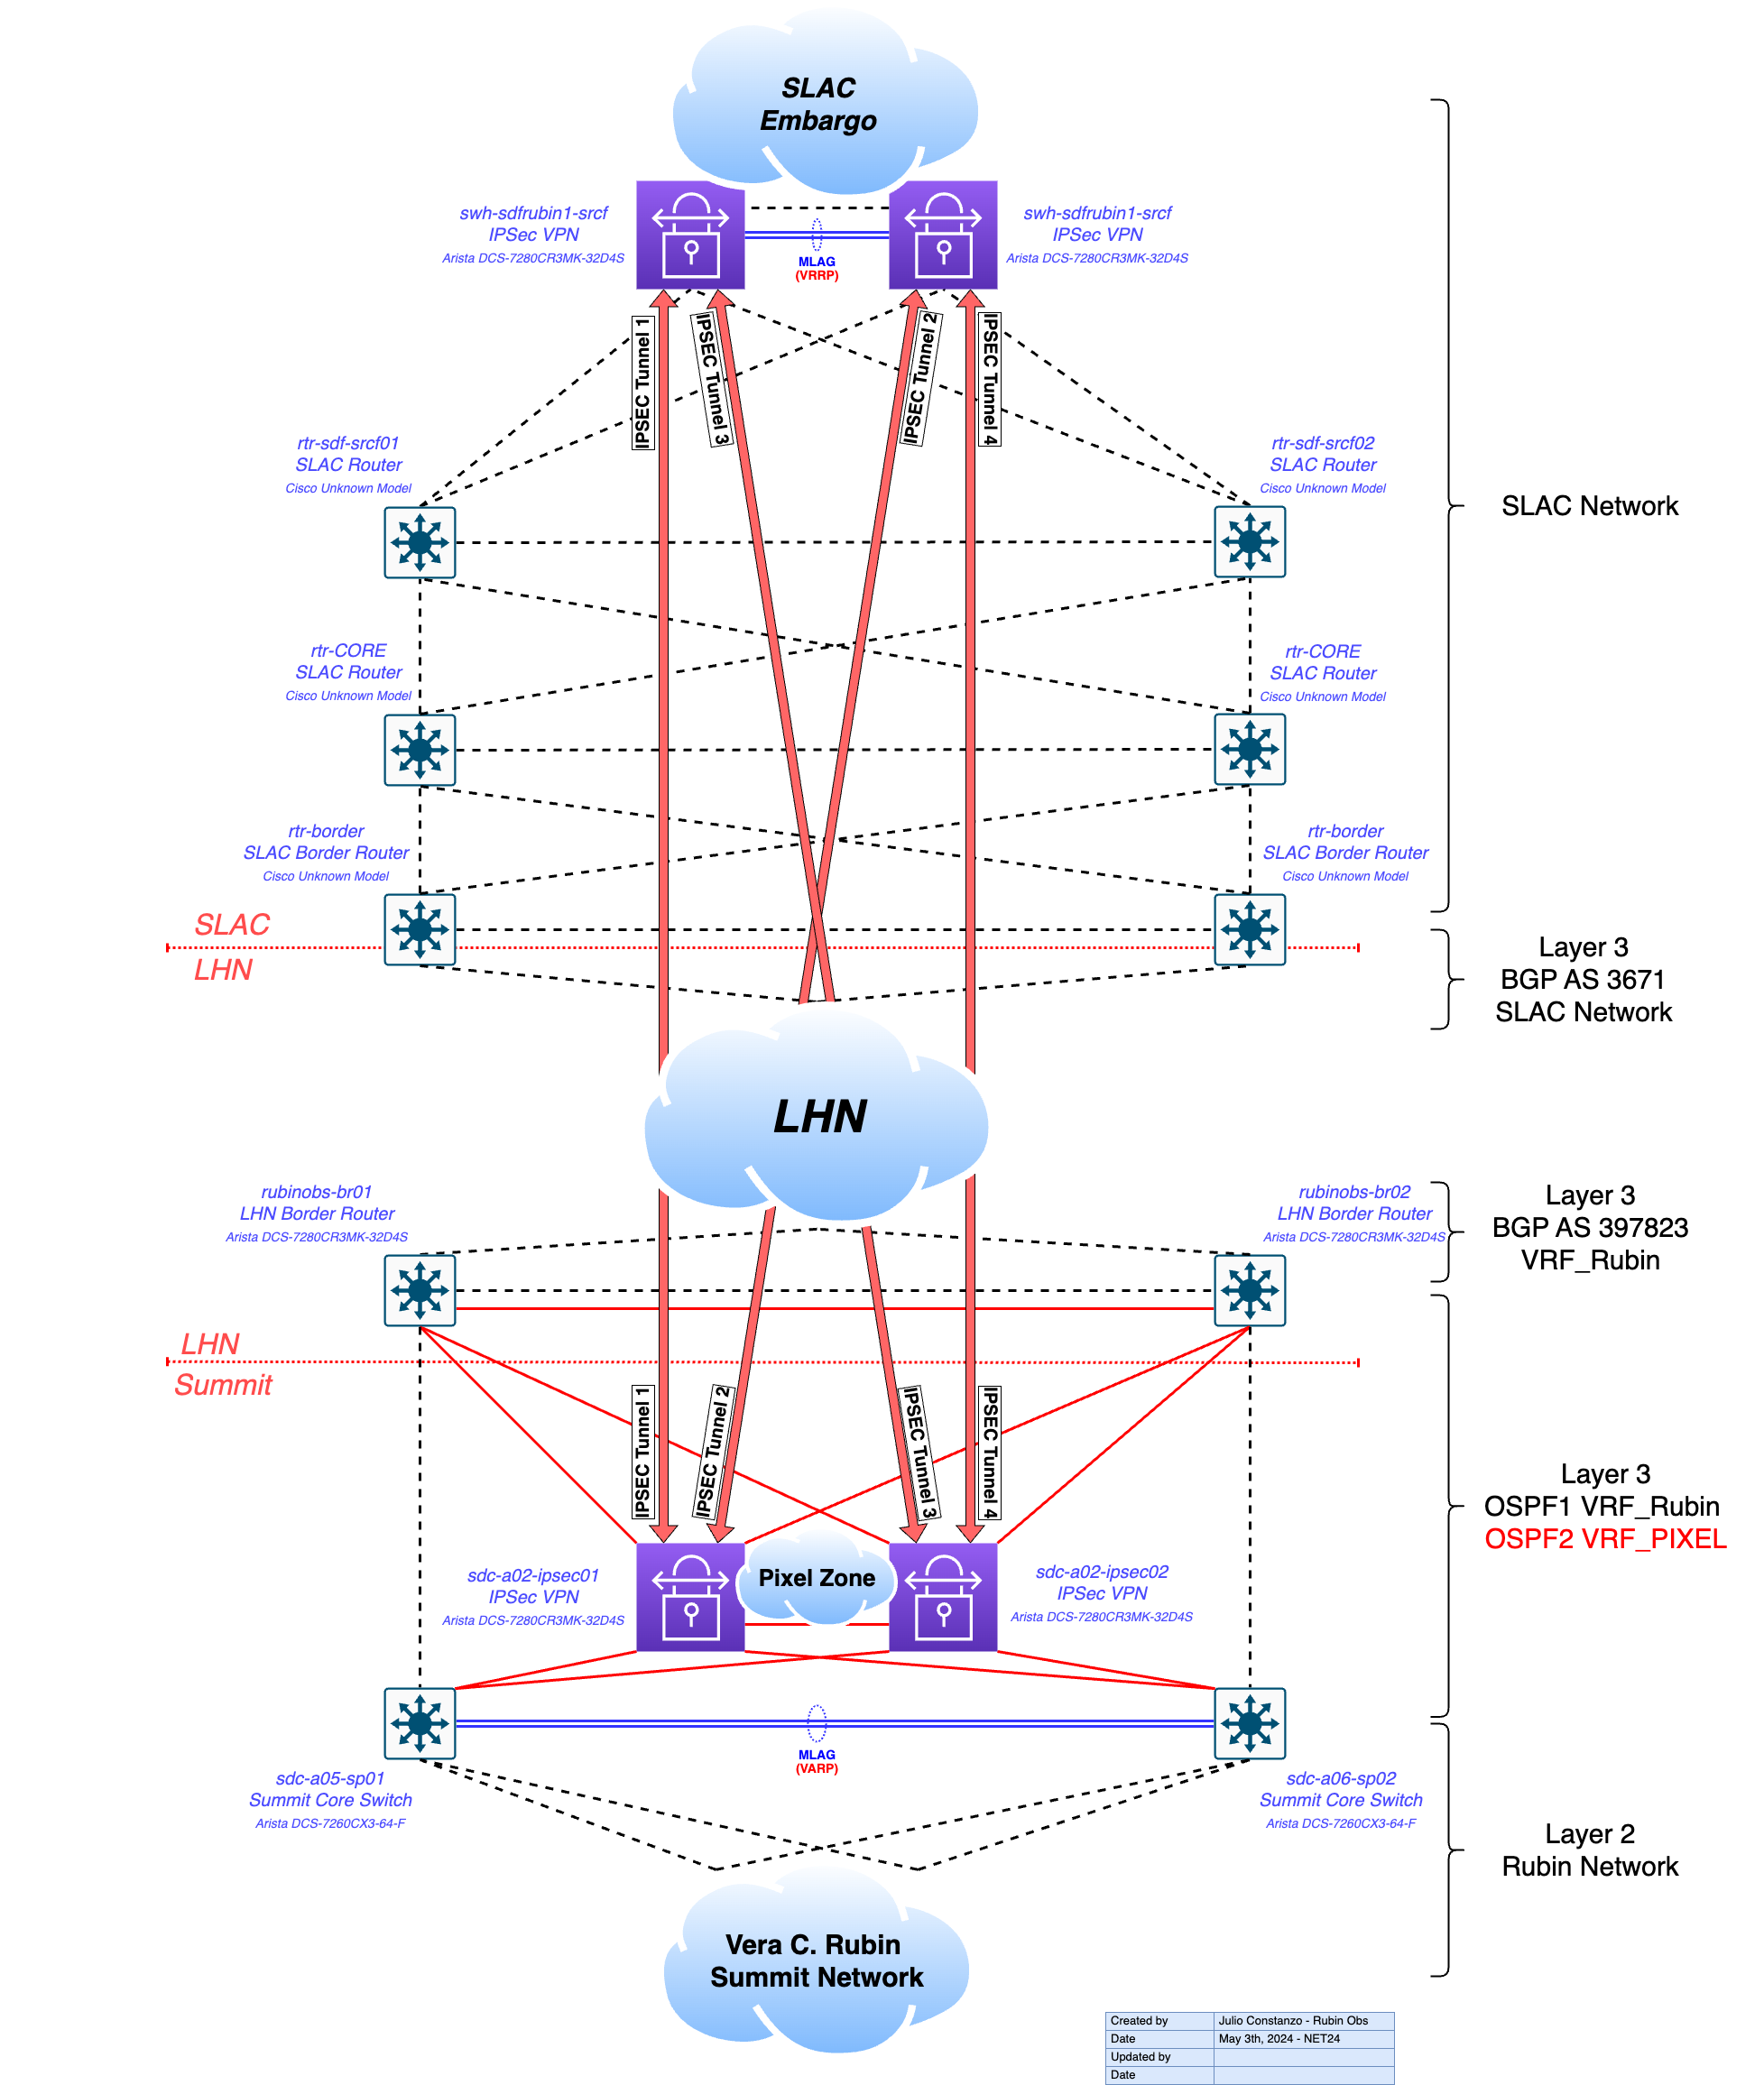
\includegraphics[width=16cm]{images/IPSec_Rubin_to_SLAC.png}
    \centering
    \caption{IPSEC Rubin to SLAC}
  \end{figure}
